\chapter{Evaluation} \label{chap:Evaluation}
This chapter presents the evaluation of the CRI extension. The goal of this is to determine how well the CRI works while debugging and understanding reactive web applications. All the applications used to evaluate the extension are taken from the internet, and they are built on RxJS or Bacon.js library. 
The first section defines a methodology for the evaluation and applies it to the pool of applications. The second section presents various case studies in detail, which demonstrate the use of the extension. Every subsection of the second section focuses on one feature and evaluates that feature with real applications. One application from both RxJS and Bacon.js is evaluated in every subsection. In the third section, some advanced web applications are debugged with CRI to check the robustness of CRI. The last section summarises and concludes the evaluation.


\section{Feasibility of the Technical Approach}

This section presents the evaluation and its result that was performed by assessing the feasibility of the technical
approach. The goal is to determine how well CRI works together with real applications. We take 22 reactive web applications, based on RxJS and Bacon.js library, from the internet. We run these applications and tried to debug and analyse them with CRI.

\subsection{Evaluated Web Applications}

Because RP paradigm is still new to the web domain, it was very hard to find a large number of reactive web applications for the purpose of evaluation. However, we found 22 applications for evaluation (10 applications are using Bacon.js, and the rest 12 are using RxJS library). Evaluated applications are listed in Table~\ref{table:eval_web_apps}. Along with the title of the application, we also present some details like how many lines of codes that application comprises of, how many Eventstreams or Observables are defined, and the number of used operators. More details of the evaluated applications are available in Appendix~\ref{chap:Appendix}.

As we have already seen in chapter 4, we are using Jalangi for instrumenting JavaScript code before executing it in the browser. Because jalangi does not support ``\textbf{arrow functions}'' (which comes as a new feature in  ECMAScript 6 and is the new syntax of writing functions in JavaScript), we replaced the arrow function syntax with normal syntax from applications before the evaluation.
Another important fact is that CRI only supports from version 5 of RxJS which is still very new. So some applications were based on earlier versions of RxJs, we modified those to make them work with version 5 before performing the evaluation.

\begin{table}[h!]
\begin{center}
	\begin{tabular}{  |c|m{4cm}|c|c|c|c|m{2cm}|}
		\hline
		No. & Application Title & Library & Code Lines & Streams & Unique Operators & Total Operators  \\ \hline
		1  & Operators and Events & Bacon.js & 74 & 8 & 7 & 15 \\ \hline
		2 & Father-Son Wallet War & Bacon.js & 19 & 2 & 3 & 5 \\ \hline
		3 & Up-Down Counter  & Bacon.js & 8 & 2 & 3 & 4 \\ \hline
		4 & Form Validation & Bacon.js & 42 & 3 & 5 & 12 \\ \hline
		5 & Movie Search & Bacon.js & 34 & 3 & 4 & 5 \\ \hline
		6 & Bar Chart & Bacon.js & 81 & 1 & 3 & 3 \\ \hline
		7 & WebSocket - Wikipedia & Bacon.js & 180 & 2 & 6 & 9 \\ \hline
		8 & Smart Counter & RxJs & 29 & 2 & 7 & 8 \\ \hline
		9 & State Sotrage & RxJs & 37 & 3 & 3 & 5 \\ \hline
		10 & Letter Counter & RxJS & 12 & 1 & 2 & 2 \\ \hline
		11 & Father-Son Wallet War & RxJS & 23 & 2 & 4 & 5 \\ \hline
		12 & Movie Search & RxJS & 33 & 2 & 2 & 5 \\ \hline
		13 & Follow The Mouse & RxJS & 45 & 1 & 8 & 2 \\ \hline
		14 & Drag and Drop  & RxJS & 19 & 3 & 3 & 3 \\ \hline
		15 & Canvas Painting & RxJS & 62 & 6 & 8 & 10 \\ \hline
		16 & Twitter Follow Box & RxJS & 57 & 5 & 5 & 8 \\ \hline
		17 & REST API Call  & RxJS & 30 & 1 & 3 & 3 \\ \hline
		18 & Spotify Artist Search & RxJS & 35 & 2 & 8 & 9 \\ \hline
		19 & Image Sampler & RxJS & 38 & 2 & 2 & 3 \\ \hline
		20 & Mullti Select Cards & Bacon.js & 79 & 3 & 5 & 15 \\ \hline
		21 & True - False Logger & Bacon.js & 44 & 7 & 5 & 16 \\ \hline
		22 & Drawing App & Bacon.js & 38 & 4 & 4 & 4 \\ \hline
		
		
	
	\end{tabular}
\end{center}

\caption{Evaluated Web Applications}
\label{table:eval_web_apps}
\end{table}


\subsection{Evaluation Criteria}
We prepared a recipe for the evaluation that comprises of eight questions. The primary goal of these questions was to see whether the use of the CRI benefits the developer to understand and to find bugs in the target application. The summary of evaluation criteria is listed in Table~\ref{table:eval_criteria}. 
First of all, we evaluated if the behaviour of the target application remains unchanged while debugging it with the CRI.  Secondly, we saw whether the CRI was able to model the target application into a dependency graph. Next, we observed that if the propagation of changes through nodes of the dependency graph are visible to the developer.
We navigated through the history of the dependency graph for the target application to see if that helped us to understand the target application better. The fifth point in the evaluation recipe is to test RP specific breakpoints. 
The next three steps are to gather some statistics about the outcomes of the CRI like getting the total number of nodes in the dependency graph, the total number of green nodes that represents the identified streams assigned to JS variables and the number of steps recorded while debugging.



\begin{table}[h!]
\begin{center}
	\begin{tabular}{  |c|m{16cm}|}
		\hline
		Q1 & While the CRI was active, did the target application run as it was running before?  \\ \hline
		Q2 & Did the CRI deliver the dependency graph of the target application?  \\ \hline
		Q3 & Was the propagation of changes to the dependency graph be visible?  \\ \hline
		Q4 & Did traversing through the history of the dependency graph helps to understand the working of target application?  \\ \hline
		Q5 & Did the execution of application pause, when we set a reactive breakpoint?  \\ \hline
		Q6 & What is the total number of nodes in the dependency graph?  \\ \hline
		Q7 & What is the total number of green nodes in the dependency graph?  \\ \hline
		Q8 & What is the total number of recorded steps?  \\ \hline
	\end{tabular}
\end{center}
\caption{Evaluation Criteria}
\label{table:eval_criteria}
\end{table}
		
\subsection{Evaluation Results}

\begin{table}[h!]
	\begin{center}
		\begin{tabular}{  |c|c|c|c|c|c|c|c|c|}
			\hline
			& Q1 & Q2 & Q3 & Q4 & Q5 & Q6 & Q7 & Q8 \\ \hline
			App-1 & Yes & Yes & Yes & Yes & Yes & 35 & 4 & 140 \\ \hline
			App-2 & Yes & Yes & Yes & Yes & Yes & 7 & 7 & 21+ \\ \hline
			App-3 & Yes & Yes & Yes & Yes & Yes & 6 & 5 & 16+ \\ \hline
			App-4 & Yes & Yes & Yes & Yes & Yes & 19 & 9 & 50+ \\ \hline
			App-5 & Yes & Yes & Yes & Yes & Yes & 42 & 5 & 125+ \\ \hline
			App-6 & Yes & Yes & Yes & Yes & Yes & 4 & 5 & 16+ \\ \hline
			App-7 & Yes & Yes & Unstable & Unstable & Yes & 14 & 15 & 20+ \\ \hline
			App-8 & Yes & Yes & Unstable & Unstable & Unstable & 7 & 0 & 16+ \\ \hline
			App-9 & Yes & Yes & Yes & Yes & Yes & 8 & 4 & 23+ \\ \hline
			App-10 & Yes & Yes & Yes & Yes & Yes & 3 & 4 & 27+ \\ \hline
			App-11 & Yes & Yes & Yes & Yes & Yes & 8 & 5 & 25+ \\ \hline
			App-12 & Yes & Yes & Yes & Yes & Yes & 6 & 6 & 21+ \\ \hline
			App-13 & Yes & Yes & Yes & Yes & Yes & 9 & 3 & 27+ \\ \hline
			App-14 & Yes & Yes & Yes & Yes & Yes & 8 & 4 & 7+ \\ \hline
			App-15 & Yes & Yes & Yes & Yes & Yes & 19 & 7 & 55+ \\ \hline
			App-16 & Yes & Yes & Yes & Yes & Yes & 32 & 9 & 134+ \\ \hline
			App-17 & Yes & Yes & Yes & Yes & Yes & 4 & 1 & 30+ \\ \hline
			App-18 & Yes & Yes & Yes & Yes & Yes & 9 & 5 & 29+ \\ \hline
			App-19 & Yes & Yes & Yes & Yes & Yes & 5 & 2 & 11+ \\ \hline
			App-20 & Yes & Yes & Yes & Yes & Yes & 54 & 6 & 118+ \\ \hline
			App-21 & Yes & Yes & Yes & Yes & Yes & 17 & 8 & 37+ \\ \hline
			App-22 & Yes & Yes & Yes & Yes & Yes & 13 & 4 & 50+ \\ \hline
			
			
	\end{tabular}
\end{center}
\caption{Evaluation Results}
\label{table:eval_results}
\end{table}

We performed the evaluation recipe, one by one to all of the applications listed in Table~\ref{table:eval_web_apps}.  Table~\ref{table:eval_results} summarises the results of the evaluation. 
For application 7 and 8, the results are unstable, and this is because these applications contain observables that emit values after a very short time interval. The CRI tries to log all events and sends a message to the panel to update values to corresponding nodes of the dependency graph. 
In the case of application 7, there is a web socket connection, and the application receives all incoming updates and afterwards samples them with a sampling interval of 2 seconds. So while debugging this application, the stream that receives updates from the web socket connection also gets subscribed which then cause high resource consumptions and leads to an uncertain behaviour.
In the case of application 8, there is an observable that emits values after every 20 milliseconds and causes high resource consumption because the extension communicate with panel after every 20 miliseconds. 

To reproduce the evaluation, one should follow the following steps:

\begin{itemize}
	\item Get and set up the target application. See Appendix~\ref{chap:Appendix} for more information for each application.
	
	\item Run the application without activating CRI extension to understand and observe its working.
	
	\item Check Appendix~\ref{chap:Appendix} for the required refactoring of the target application.
	
	\item Activate the CRI extension, open \textbf{reactive inspector} panel from Chrome DevTools and execute the target application.
	
	\item Apply the evaluation criteria mentioned in Table~\ref{table:eval_criteria}.
		
	
\end{itemize}

\section{Case Studies}
In this section, various case studies are presented in detail, which demonstrate the use of the CRI extension. They have been chosen in order to illustrate the most important features of the extension. The goal of these case studies is to show how a developer new to RP could use  the CRI to understand the target application and solve potentially complex problems. The case studies do not fix the bugs in the target application but often lead the developer into a direction to understand and find the bugs quickly.



\subsection{Understanding Operators}

Operators provided by reactive libraries has already been presented in section~\ref{subsec:Operators}. While developing reactive applications, one needs to use different operators for transforming, combining, filtering, mathematical operations. To chose the correct operator, one needs to understand its workings in detail. The CRI helps the developer to understand the abstract workings of operators. We used some operators provided by RxJs and Bacon libraries in the sample application and then tried to use the CRI to understand the working details of those operators. This section illustrates how the CRI helps to understand the working details of operators provided by reactive libraries with sample applications.

\subsubsection{Bacon.js - Operators}

Listing~\ref{lst:evaluation-bacon-opr} shows a sample application that uses the filter, fold and scan operators of Bacon.js library. From line 1 to 13 in the source code, the usage of filter operator is shown. Line 5 uses \textbf{sequentially} to create a stream containing given values from an array delivered with a given interval in milliseconds. Line 6 to 8 apply filter operator on the created stream to filter odd values from the array, that results in a stream of values. Line 9 to 11 is the subscription of the filtered stream.
Line 15 to 23,  \textbf{fold} operator is used to calculate the sum of all elements of the array. Line 25 to 33,  \textbf{scan} operator is used to calculate the sum of all elements of the array. Figure~\ref{fig:bacon-operators-dg-with-ui} shows the dependency graph of the target application of listing~\ref{lst:evaluation-bacon-opr}. When we click on the button \textbf{Run (filter)}, the filter operation can be observed in the dependency graph created by the CRI. Two nodes on the top represent filter operation. The first node represents the source stream that emits values from the array one by one after every 1000 milliseconds. The second node represents the filtered stream that emits only even values.
On hovering over the node, a popup opens up with detailed information about that particular node. 
According to Bacon.js API documentation\footnote{\url{https://baconjs.github.io/api.html} , last accessed 22-05-2017}, fold operator is like \textbf{scan} operator but only emits the final value. This behaviour can be easily visualised in the dependency graph.


\begin{lstlisting}[language=JavaScript, caption=Understanding Bacon.js Operators, label={lst:evaluation-bacon-opr}]
// Array data source
var arr = [1, 2, 3, 4, 5, 6, 7, 8, 9, 10];
// Filter
$("#runBaconFilter").click(function () {
	var baconSourceStream = Bacon.sequentially(1000, arr);
	var baconFilteredEvenStream = baconSourceStream.filter(function (x) {
	return x % 2 == 0;
});
baconFilteredEvenStream.onValue(function (val) {
	$("#baconFilter").text(val);
});

});
// Sum of array elements with Fold
$("#runBaconFold").click(function () {
	var baconStream = Bacon.sequentially(500, arr);
	var baconFoldStream = baconStream.fold(0, function (x, acc) {
	return x + acc;
});
baconFoldStream.onValue(function (val) {
	$("#baconFold").text(val);
});
});
// Sum of array elements with Scan
$("#runBaconScan").click(function () {
	var baconStream = Bacon.sequentially(500, arr);
	var baconScanStream = baconStream.scan(0, function (x, acc) {
	return x + acc;
});
baconScanStream.onValue(function (val) {
	$("#baconScan").text(val);
});
});
\end{lstlisting}



\begin{figure}[!h]
	\centering
	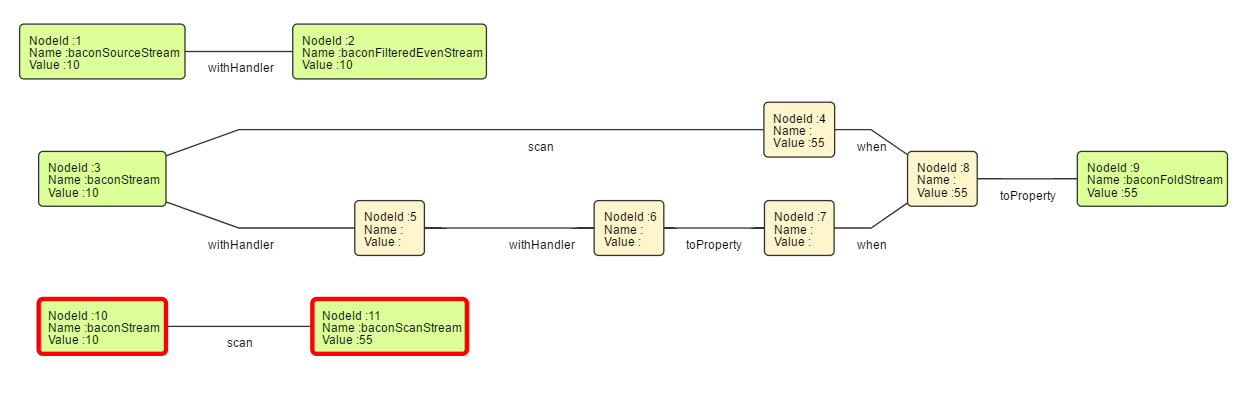
\includegraphics[width=\textwidth,height=\textheight,keepaspectratio]{gfx/evaluation/dg_bacon-operators.png}
	\caption{Dependency Graph of Bacon.js Operators}
	\label{fig:bacon-operators-dg-with-ui}
\end{figure}


\subsubsection{RxJS - Operators}
Listing~\ref{lst:evaluation-rxjs-opr} shows a sample application that makes use, \textbf{mapTo}, \textbf{delay} and \textbf{merge} operators from RxJS library. When the program is executed, the dependency graph created by the CRI is shown in figure~\ref{fig:rxjs-operator-delay}. The dependency graph shows four observables emitting different strings with a specified delay value. Merging these four observables then results in a desired observable which is assigned to a variable called \textbf{\textit{message}}. A subscriber of the resultant observable receives a string of values one by one with a specified delay.

\begin{lstlisting}[language=JavaScript, caption=Understanding RxJS Operators, label={lst:evaluation-rxjs-opr}]
//emit one item
var example = Rx.Observable.of(null);
//delay output of each by an extra second
var message = Rx.Observable.merge(
	example.mapTo('Hello'),
	example.mapTo('World!').delay(1000),
	example.mapTo('Goodbye').delay(2000),
	example.mapTo('World!').delay(3000)
);
//output: 'Hello'...'World!'...'Goodbye'...'World!'
var subscribe = message.subscribe(function (val) {
	return console.log(val);
});
\end{lstlisting}

\begin{figure}[!h]
	\centering
	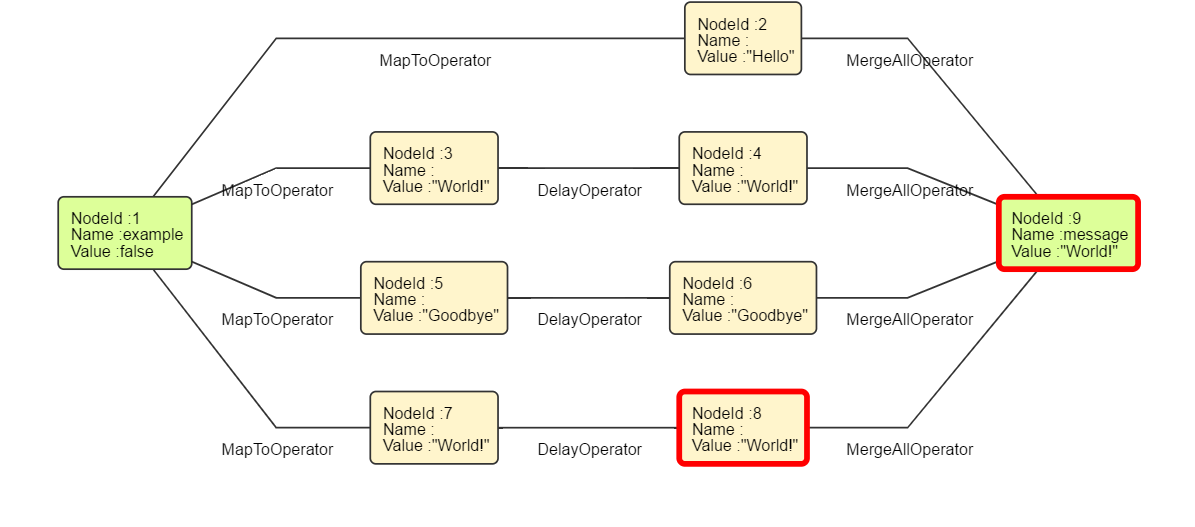
\includegraphics[width=\textwidth,height=\textheight,keepaspectratio]{gfx/evaluation/rxjs-operator-delay.png}
	\caption{Dependency Graph of Bacon.js Operators}
	\label{fig:rxjs-operator-delay}
\end{figure}

\subsection{Understanding Reactive Systems with Dependency Graph History}

Besides modelling the reactive applications into a dependency graph, the storage of the whole dependency graph history and the possibility navigating through it are the important features of the CRI. One can use a simple slider to navigate through the history of the dependency graph as described in Section~\ref{Graphical_User_Interface}. With this navigation feature, one can see the evolution of the shape of the dependency graph. One can see how nodes are created and how dependencies are established. One can also observe how changes propagate through the dependency graph. The above mentioned features help to comprehend the execution of the reactive application step-by-step and dependencies among reactive variables are easily visible. Doing this with a native DevTools would potentially mean that it jumps around in the source code so that one cannot comprehend the steps at all. With the help of the dependency graph visualisation, the steps are easily comprehensible and shown in a more natural format. 
This section will further evaluate these features with some sample applications.

\subsubsection{Bacon.js - Up-Down Counter}

Listing~\ref{lst:evaluation-bacon-udc} presents the relevant source code of an up-down counter application  based on Bacon.js. GUI of this application contains two buttons (up and down) and one DOM element to display the final result. Figure~\ref{fig:bacon_up_down_counter_evolution} shows the evolution of the dependency graph when the target application is run by activating the CRI extension. Figure~\ref{fig:bacon_up_down_final} represent the state of the dependency graph when the user clicks twice on the DOM element with id \textbf{up}. The complete application can be easily overviewed with the dependency graph. One can easily see that two streams are being merged and scan to deliver desired results. 

\begin{lstlisting}[language=JavaScript, caption=Bacon.js - Up-Down Counter, label={lst:evaluation-bacon-udc}]
var up = $('#up').asEventStream('click');
var down = $('#down').asEventStream('click');
var upClick = up.map(1);
var downClick = down.map(-1);
var counter = upClick.merge(downClick).scan(0, function (x, y) {
	return x + y;
});
counter.assign($('#counter'), 'text');
\end{lstlisting}


\begin{figure}[!h]
	\centering
	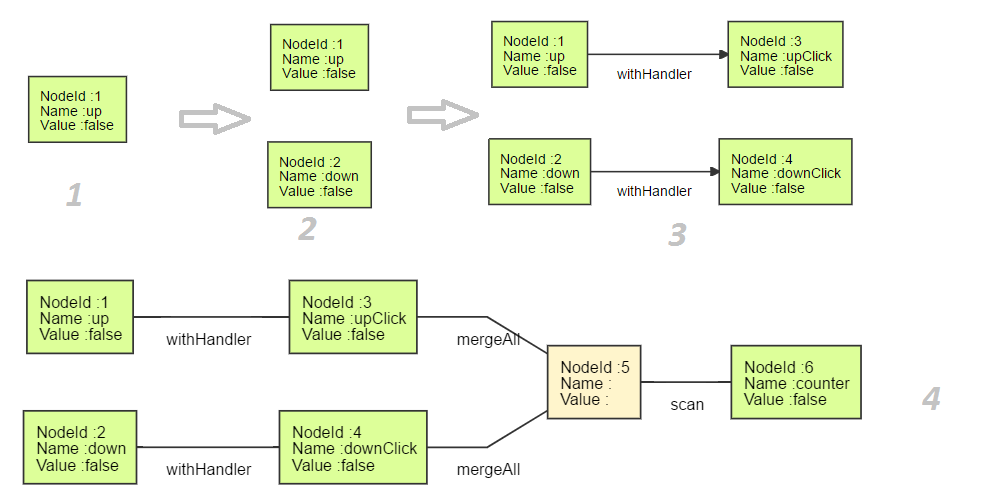
\includegraphics[width=\textwidth,height=\textheight,keepaspectratio]{gfx/evaluation/bacon_up_down_counter_evolution.png}
	\caption{Up-Down Counter - Evolution of the Dependency Graph}
	\label{fig:bacon_up_down_counter_evolution}
\end{figure}


\begin{figure}[!h]
	\centering
	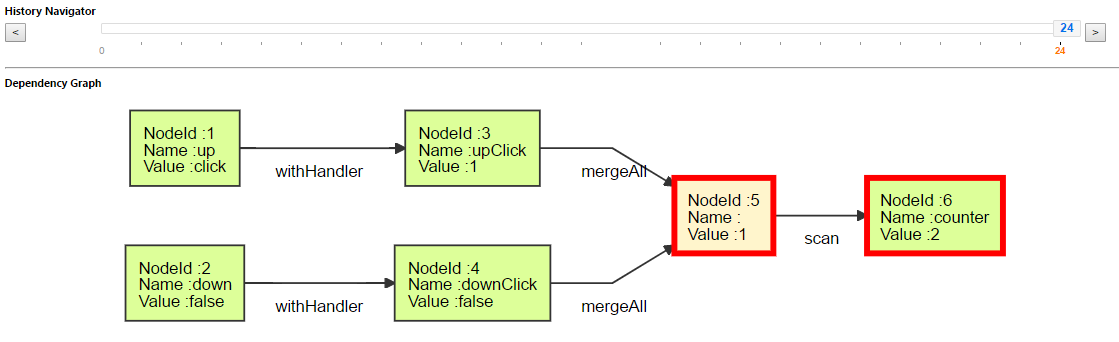
\includegraphics[width=\textwidth,height=\textheight,keepaspectratio]{gfx/evaluation/bacon_up_down_final.png}
	\caption{Bacon.js - Up-Down Counter}
	\label{fig:bacon_up_down_final}
\end{figure}

\subsubsection{RxJS - State Management}

Let us look at another case from RxJS applications. This application manages the state of three DOM elements. The relevant code is in Listing~\ref{lst:evaluation-rxjs-statemgmt}.  The \textbf{state} object comprises of \textbf{count} and \textbf{inputValue}. The \textbf{count} attribute of the state object is linked to two buttons, which increase and decrease the count value. \textbf{inpuValue} is the current value of a text field.  The dependency graph of this application is depicted in figure~\ref{fig:rxjs_state_save}. One can clearly see in the dependency graph that three streams are being merged. The resultant stream is scanned to get the required stream which always emits the current state of the system on any change in the values of relevant DOM elements.

\begin{lstlisting}[language=JavaScript, caption=RxJS - State Management, label={lst:evaluation-rxjs-statemgmt}]
var increaseButton = document.querySelector('#increase');
var increase = Rx.Observable.fromEvent(increaseButton, 'click')
// Again we map to a function the will increase the count
.map(function () {
	return function (state) {
		return Object.assign({}, state, { count: state.count + 1 });
	};
});

var decreaseButton = document.querySelector('#decrease');
var decrease = Rx.Observable.fromEvent(decreaseButton, 'click')
// We also map to a function that will decrease the count
.map(function () {
	return function (state) {
		return Object.assign({}, state, { count: state.count - 1 });
	};
});

var inputElement = document.querySelector('#input');
var input = Rx.Observable.fromEvent(inputElement, 'keyup')
// Let us also map the keypress events to produce an inputValue state
.map(function (event) {
	return function (state) {
		return Object.assign({}, state, { inputValue: event.target.value });
	};
});

// We merge the three state change producing observables
var state = Rx.Observable.merge(increase, decrease, input).scan(function (state, changeFn) {
	return changeFn(state);
}, {
count: 0,
inputValue: ''
});

// We subscribe to state changes and update the DOM
// has actually changed
var prevState = {};
state.subscribe(function (state) {
	if (state.count !== prevState.count) {
		document.querySelector('#count').innerHTML = state.count;
	}
	if (state.inputValue !== prevState.inputValue) {
		document.querySelector('#hello').innerHTML = 'Hello ' + state.inputValue;
	}
prevState = state;
});
\end{lstlisting}



\begin{figure}[!h]
	\centering
	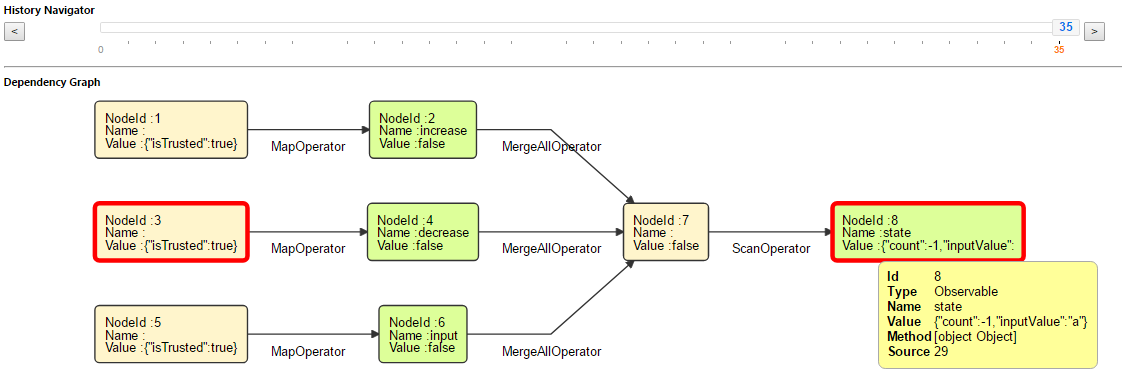
\includegraphics[width=\textwidth,height=\textheight,keepaspectratio]{gfx/evaluation/rxjs_state_save.png}
	\caption{RxJS - Dependency Graph of State Management}
	\label{fig:rxjs_state_save}
\end{figure}

\subsection{Querying the Dependency Graph History}
In this section, we show how the developer can query the history of the dependency graph using query language presented in chapter~\ref{chap:Implementation}. The developer can use this feature either to find bugs in the application or to observe the data flow through different nodes of the dependency graph. First, we execute the program and then we query the dependency graph history.

\subsubsection{Bacon.js - Father and Son Wallet War}

Let\textquotesingle s now look at an interesting application called \textbf{Father and Son Wallet War}. This application is based on a rule that the father will always have ten dollars more than his son. The initial value of father wallet is ten. Figure~\ref{fig:son_father_wallet_ui} is a screenshot of the GUI of the application. Listing~\ref{lst:evaluation-bacon-son-father-wallet} show the relevant source code of this application. When we execute this application, the CRI extension models it into the dependency graph in 21 steps. Then we have done the following series of actions on the application \textbf{+ , + , + , - , + , + , + , - , - , +}  (where \textbf{+} represent one click on \textbf{Add 1 to son} and \textbf{-} represent one click on \textbf{Remove 1 from  son} button)
Figure~\ref{fig:bacon_son_father_wallet_war} show the state of the dependency graph after applying this series of actions.
Then we ran the following query to \textbf{History Queries} section of the CRI.  \textbf{evaluationYielded[sonWalletValue][3]}
We found three results that matched our query where the son wallet value was three at step 36 , 46 and 66.
Now we want to know that during execution of the program, how many node \textbf{addClickMap} results to 1, we execute the following query for that \textbf{evaluationYielded[addClickMap][1]}, which gives us 7 results, so it means add click button was clicked 7 times, which is true. 



\begin{figure}[!h]
	\centering
	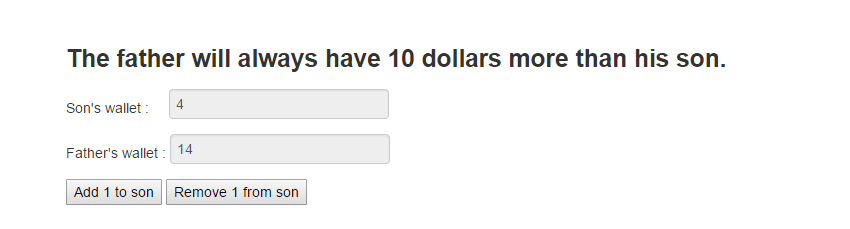
\includegraphics[width=\textwidth,height=\textheight,keepaspectratio]{gfx/evaluation/son_father_wallet_ui.png}
	\caption{GUI - Father And Son Wallet War}
	\label{fig:son_father_wallet_ui}
\end{figure}

\begin{lstlisting}[language=JavaScript, caption=Bacon.js - Father And Son Wallet War, label={lst:evaluation-bacon-son-father-wallet}]
$sonWallet = $('#wallet-son');
$fatherWallet = $('#wallet-father');
$addSon = $('#add-son');
$removeSon = $('#remove-son');

// change the value in the son's wallet
addClick = $addSon.asEventStream('click');
addClickMap = addClick.map(1);
removeClick = $removeSon.asEventStream('click');
removeClickMap = removeClick.map(-1);

eventClick = addClickMap.merge(removeClickMap);
function plus(a, b) {
	return a + b
}
sonWalletValue = eventClick.scan(0, plus)
fatherWalletValue = sonWalletValue
.map(function (value) {
	return value + 10
})
sonWalletValue.assign($sonWallet, "val");
fatherWalletValue.assign($fatherWallet, "val");
\end{lstlisting}

\begin{figure}[!h]
	\centering
	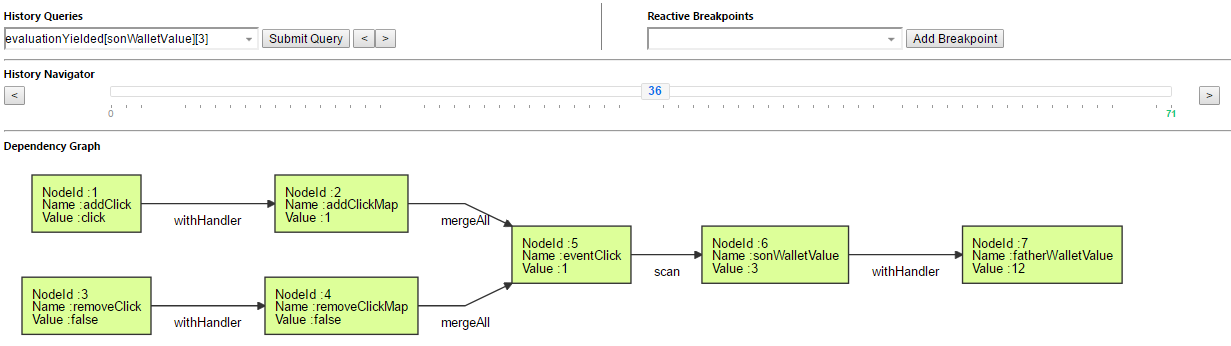
\includegraphics[width=\textwidth,height=\textheight,keepaspectratio]{gfx/evaluation/bacon-dg_son_father_wallet_search.png}
	\caption{History Query - Father And Son Wallet War}
	\label{fig:bacon_son_father_wallet_war}
\end{figure}



\subsubsection{RxJS - Movie Search}
Listing~\ref{lst:evaluation-rxjs_movie_search} shows a Movie Search application that makes HTTP GET request to the third party server and shows the results on the target page. Figure~\ref{fig:rxjs_movie_search} shows the GUI of the target application. Keyup event on the text field is mapped to get the value of the text field, which is further filtered for checking the minimum length. \textbf{debounceTime} operator is used to limit the number of requests to the server. It emits values only after 750ms have passed since it emitted last time.
Figure~\ref{fig:rxjs_movie_search_dg} shows the dependency graph of the target application. While debugging this application, we search through the history of the dependency graph using the query language to see what values at node \textbf{afterDebounce} are received and then we can easily adjust the debounce time value accordingly. 


\begin{lstlisting}[language=JavaScript, caption=RxJS - Movie Search, label={lst:evaluation-rxjs_movie_search}]
// Search Movies for a given term
function searchMovie(query) {
	return jQuery.get(
		'//api.themoviedb.org/3/search/movie?api_key=9eae05e667b4d5d9fbb75d27622347fe&query=' + query
		).then(function (r) {
		return r.results;
	});
}
var $input = $('#textInput');
// Get all distinct key up events from the input
// and only fire if long enough and distinct
var keyup = Rx.Observable.fromEvent($input, 'keyup');
var mappedValue = keyup.map(function (e) {
	return e.target.value; // Project the text from the input
});
var filteredValue = mappedValue.filter(function (text) {
	return text.length > 2; // Only if the text is longer than 2 characters
});
var afterDebounce = filteredValue.debounceTime(750 /* Pause for 750ms */);
var distinctUntilChnaged = afterDebounce.distinctUntilChanged(); // Only if the value has changed
// Final Stream
var searcher = distinctUntilChnaged.switchMap(searchMovie);
\end{lstlisting}

\begin{figure}[!h]
	\centering
	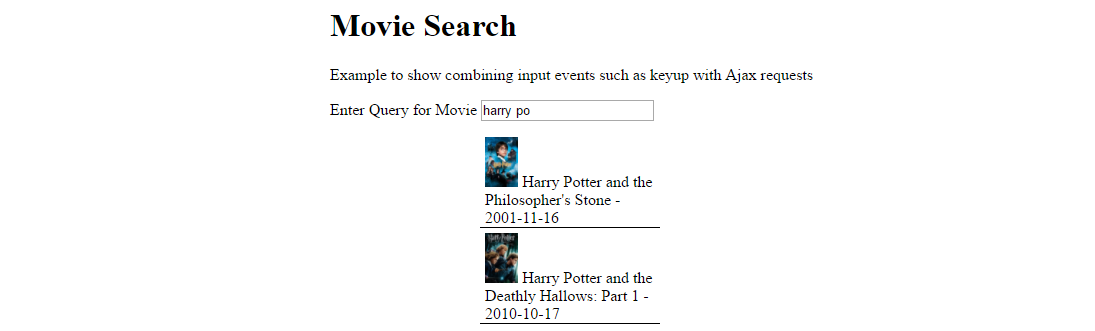
\includegraphics[width=\textwidth,height=\textheight,keepaspectratio]{gfx/evaluation/movie_search_ui.png}
	\caption{RxJS - Movie Search UI}
	\label{fig:rxjs_movie_search}
\end{figure}

\begin{figure}[!h]
	\centering
	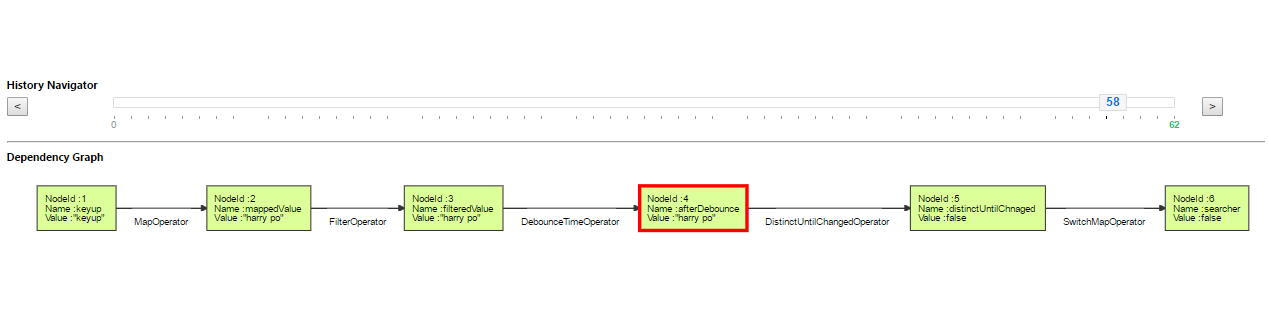
\includegraphics[width=\textwidth,height=\textheight,keepaspectratio]{gfx/evaluation/rxjs_movie_search_history.png}
	\caption{RxJS - Dependency Graph of Movie Search}
	\label{fig:rxjs_movie_search_dg}
\end{figure}




\subsection{Reactive-Programming-Specific Breakpoints}

For fast-running applications with a short life cycle, it is not a problem to find an interesting point in the history of the dependency graph after the program has completed its execution. There are situations where programs either take a 
long time to execute or the occurrence of the interesting event is uncertain. In such cases, it is very important to be able to have the possibility to define queries beforehand and the debugger halts the execution once a matching result occurs. 
This feature has been discussed before as the reactive-programming-specific breakpoints feature. In this section, we illustrate this with a few real applications. Before the program is executed, the query is defined. Then, the debugger is started as before. It will then pause the execution each time it matches to the defined queries. Let\textquotesingle s have a look at a few applications to evaluate this feature.

\subsubsection{Bacon.js - Registration Form}

This application implements form validation logic in a reactive way. This application validates the availability of a username from the server by sending Ajax request. The full name field is also mandatory. 
Figure~\ref{fig:bacon_reg_form_ui} shows the GUI of this application, the left-hand side shows the case where the given username is not available.  The user gets a message about the unavailability of the username and the submit button remains disabled. The right side shows the case where the entered username is available and the full name is also given, so the submit button is enabled. 

\begin{figure}[!h]
	\centering
	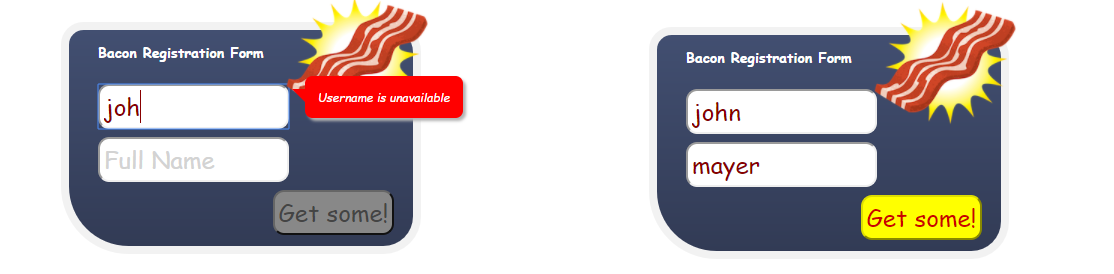
\includegraphics[width=\textwidth,height=\textheight,keepaspectratio]{gfx/evaluation/bacon_reg_form_ui.png}
	\caption{Bacon.js - GUI of Registration Form}
	\label{fig:bacon_reg_form_ui}
\end{figure}



Listing~\ref{lst:evaluation-bacon_regform} shows the source code of the target application. Figure~\ref{fig:bacon_dg_regform} shows the dependency graph in the state when the form is validated and the submit button is enabled. We have observed a case where the entered username is available and full name is also given but still, the submit button is not enabled. We tried to debug this issue with the CRI extension. For this, we set a reactive break point by defining a query \textbf{evaluationYeilded[3][false]}. While executing, we noticed that as soon as user typed any character from \"a, \"o or \"u , the node with id 3 emit false. Figure 5.12 shows the screenshot of the debugging session where the program execution paused by the reactive breakpoint.  We looked into the relevant code and found that there is a restriction of umlaut characters. 

\begin{figure}[!h]
	\centering
	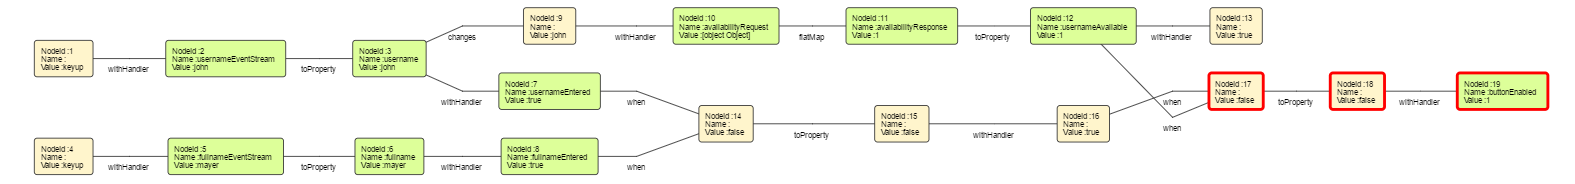
\includegraphics[width=\textwidth,height=\textheight,keepaspectratio]{gfx/evaluation/bacon_dg_regform.png}
	\caption{Bacon.js - Dependency Graph of Registration Form Application}
	\label{fig:bacon_dg_regform}
\end{figure}

\begin{lstlisting}[language=JavaScript, caption=Bacon.js - Registration Form, label={lst:evaluation-bacon_regform}]
function show(x) { console.log(x) }
function nonEmpty(x) { return x.length > 0 }
function setVisibility(element, visible) {
	element.toggle(visible)
}
var usernameEventStream = $("#username input").asEventStream("keyup").map(function (event) {
var typedValue = $(event.target).val();
// Umlaut Characters are not allowed
if( (typedValue.indexOf('ä') !== -1) || (typedValue.indexOf('ö') !== -1) || (typedValue.indexOf('ü') !== -1)){
	return 'false';
}else{
	return typedValue;
}
});
var username = usernameEventStream.toProperty("");
var fullnameEventStream = $("#fullname input").asEventStream("keyup").map(function (event) {
	return $(event.target).val()
});
var fullname = fullnameEventStream.toProperty("");
var usernameEntered = username.map(nonEmpty)
fullnameEntered = fullname.map(nonEmpty)
function toResultStream(request) {
	return Bacon.fromPromise($.ajax(request))
}
availabilityRequest = username.changes().map(function(user) { return { url: "/test.php?uname=" + user }});
availabilityResponse = availabilityRequest.flatMap(toResultStream)
usernameAvailable = availabilityResponse.toProperty(true)
usernameAvailable.not().onValue(function (show) {
setVisibility($("#username-unavailable"), show);
})
var buttonEnabled = usernameEntered.and(fullnameEntered).and(usernameAvailable)
//var buttonEnabled = fullnameEntered.and(usernameAvailable)
buttonEnabled.onValue(function(enabled) {
	$("#register button").attr("disabled", !enabled)
})
\end{lstlisting}

\begin{figure}[!h]
	\centering
	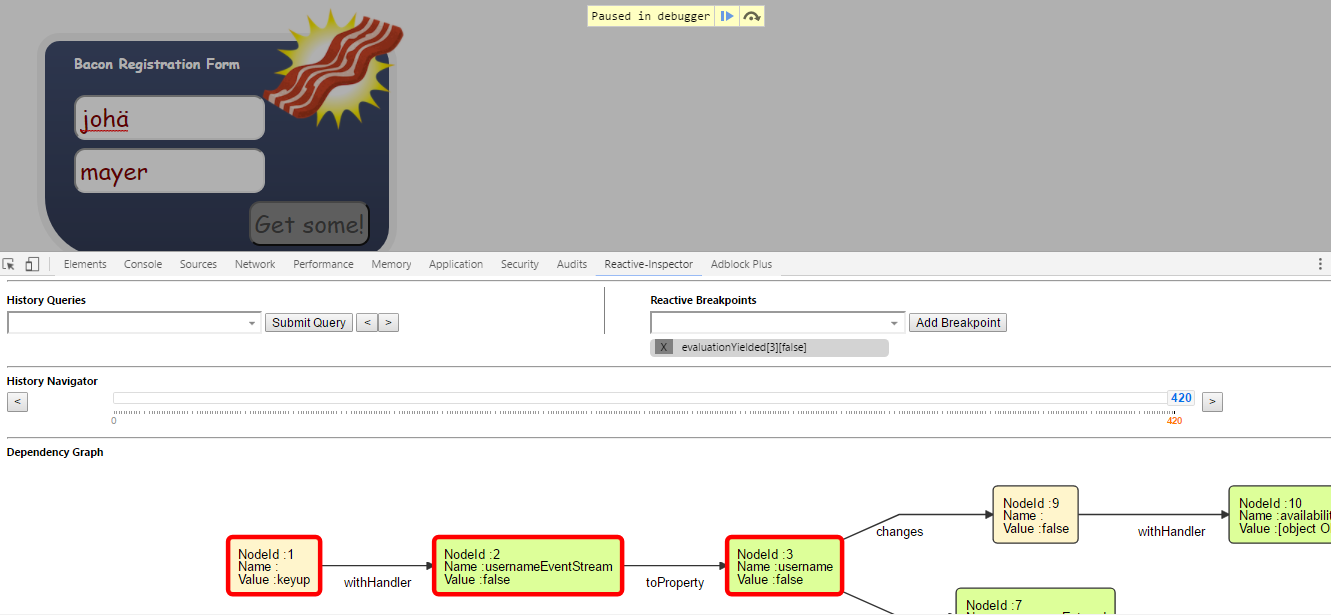
\includegraphics[width=\textwidth,height=\textheight,keepaspectratio]{gfx/evaluation/reg_form_reactive_bpoint.png}
	\caption{Bacon.js - Reactive Breakpoint in Registration Form Application}
	\label{fig:reg_form_reactive_bpoint}
\end{figure}

\subsubsection{RxJS - Follow the Mouse Pointer}

This application binds three DOM elements to the movement of the mouse pointer. Whereever the user moves the mouse pointer, those three DOM elements reposition themselves on the screen. Each DOM element changes its position with a certain delay which is defined in source code. Listing~\ref{lst:evaluation-mouse_follow} shows the source code of target application.  Figure~\ref{fig:dg_mouse_follow} depicts the dependency graph of this application, where the user can see the defined streams and operators applied to those streams. The features of reactive breakpoints can be useful in this kind of application where the application does not have a limited life cycle. 

\begin{lstlisting}[language=JavaScript, caption=RxJS - Follow the Mouse Pointer, label={lst:evaluation-mouse_follow}]
(function () {
function extractClientX(e) { return e.clientX; }
function extractClientY(e) { return e.clientY; }
function setLeft(x) { this.style.left = x + 'px'; }
function setTop(y) { this.style.top = y + 'px'; }	
function add(x, y) { return x + y; }
var partialAdd = function (x) { return add.bind(null, x); }
var delay = 300;
var mousemove = Rx.Observable.fromEvent(document, 'mousemove');
var left = mousemove.map(extractClientX);
var top = mousemove.map(extractClientY);
// Update the mouse
var themouse = document.querySelector('#themouse');
left.subscribe(setLeft.bind(themouse));
top.subscribe(setTop.bind(themouse));
// Update the tail
var mouseoffset = themouse.offsetWidth;
var thetail = document.querySelector('#thetail');
left.map(partialAdd(mouseoffset))
.delay(delay)
.subscribe(setLeft.bind(thetail));
top.delay(delay)
.subscribe(setTop.bind(thetail));
// Update wagging
var wagDelay = delay * 1.5;
var wagging = document.querySelector('#wagging');
var mouseandtailoffset = mouseoffset + thetail.offsetWidth;
left.map(partialAdd(mouseandtailoffset))
	.delay(wagDelay)
	.subscribe(setLeft.bind(wagging));
top.delay(wagDelay)
	.subscribe(setTop.bind(wagging));
}());
\end{lstlisting}

\begin{figure}[!h]
	\centering
	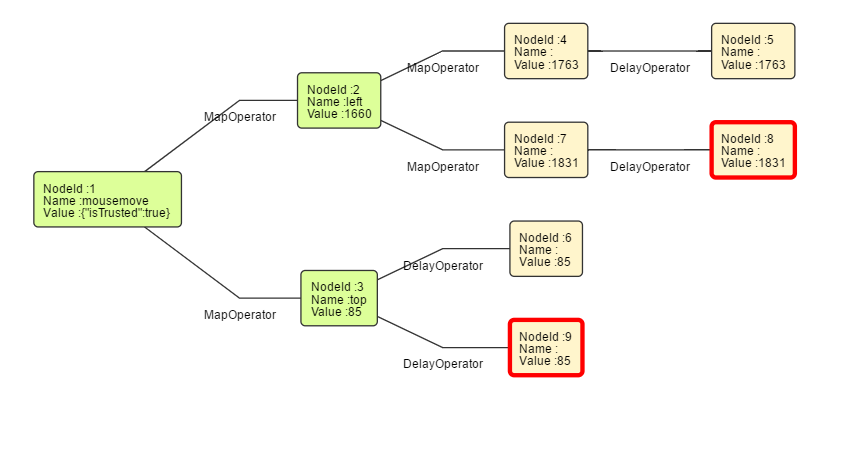
\includegraphics[width=\textwidth,height=\textheight,keepaspectratio]{gfx/evaluation/dg_mouse_follow.png}
	\caption{RxJS - Follow the Mouse Pointer}
	\label{fig:dg_mouse_follow}
\end{figure}





\section{More Advance Applications}
This section will evaluate the robustness of the CRI extension with some advanced applications.

\subsection{RxJS - Canvas Painting Board}

\begin{figure}[!h]
	\centering
	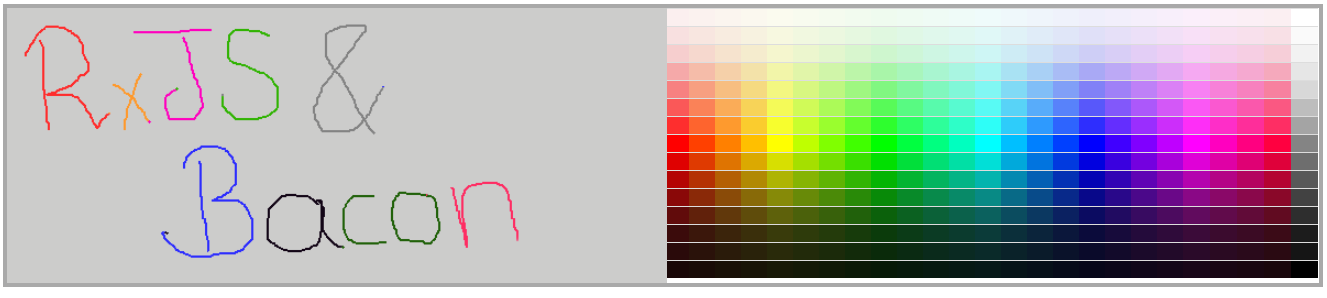
\includegraphics[width=\textwidth,height=\textheight,keepaspectratio]{gfx/evaluation/canvas_paint_ui.png}
	\caption{RxJS - Canvas Painting Board}
	\label{fig:canvas_paint_ui}
\end{figure}

This application is built with RxJS. Figure~\ref{fig:canvas_paint_ui} shows the GUI of Canvas Painting Board application. The user can select a colour and can draw on the canvas with the mouse. Listing ~\ref{lst:evaluation-canvas_paint} shows the relevant source code. The target application can easily understand by viewing its dependency graph. Figure~\ref{fig:dgraph_canvaspaint} shows a snapshot of the dependency graph. The user can easily see defined streams and applied operators. Every event while drawing something on canvas can be observed in the dependency graph. 


\begin{lstlisting}[language=JavaScript, caption=RxJS - Canvas Painting Board, label={lst:evaluation-canvas_paint}]
	Rx.DOM = {};
['mousemove', 'mouseup', 'mousedown', 'click'].forEach(function (name) {
	Rx.DOM[name] = function (element, selector) {
		return Rx.Observable.fromEvent(element, name, selector);
	};
});
Rx.DOM.ready = function () {
	return Rx.Observable.create(function (o) {
		function handler() {
			o.next();
			o.complete();
		}
		var added = false;
		if (document.readyState === 'complete') {
			handler();
		} else {
			console.log("else");
			document.addEventListener('DOMContentLoaded', handler, false);
		}
	}).take(1);
};

// Calcualte offset either layerX/Y or offsetX/Y
function getOffset(event) {
	return {
		offsetX: event.offsetX === undefined ? event.layerX : event.offsetX,
		offsetY: event.offsetY === undefined ? event.layerY : event.offsetY
	};
}

function intialize() {
	var canvas = document.getElementById('tutorial');
	var colorchart = document.querySelectorAll('#colorchart tr td');
	var ctx = canvas.getContext('2d');
	ctx.beginPath();
	
	// Get mouse events
	var mouseMoves = Rx.DOM.mousemove(canvas),
	mouseDowns = Rx.DOM.mousedown(canvas),
	mouseUps = Rx.DOM.mouseup(canvas);
	
	// Get the table events
	var colorValues = Rx.DOM.click(colorchart)
	.do(function () {
		ctx.beginPath();
	})
	.map(function (e) {
		return e.target.bgColor;
	})
	.startWith('#000000');
	
	// Calculate difference between two mouse moves
	var mouseDiffs = mouseMoves.zip(mouseMoves.skip(1), function (x, y) {
		return {first: getOffset(x), second: getOffset(y)};
	});
	
	// Get merge together both mouse up and mouse down
	var mouseButton = mouseDowns.mapTo(true)
	.merge(mouseUps.mapTo(false));
	
	// Paint if the mouse is down
	var paint = mouseButton.switchMap(function (down) {
		return down ? mouseDiffs : Rx.Observable.never();
	})
	.combineLatest(colorValues, function (pos, color) {
		return {pos: pos, color: color};
	});
	
	// Update the canvas
	paint.subscribe(function (x) {
		ctx.strokeStyle = x.color;
		ctx.moveTo(x.pos.first.offsetX, x.pos.first.offsetY);
		ctx.lineTo(x.pos.second.offsetX, x.pos.second.offsetY);
		ctx.stroke();
	});
}
Rx.DOM.ready().subscribe(intialize);
\end{lstlisting}



\begin{figure}[!h]
	\centering
	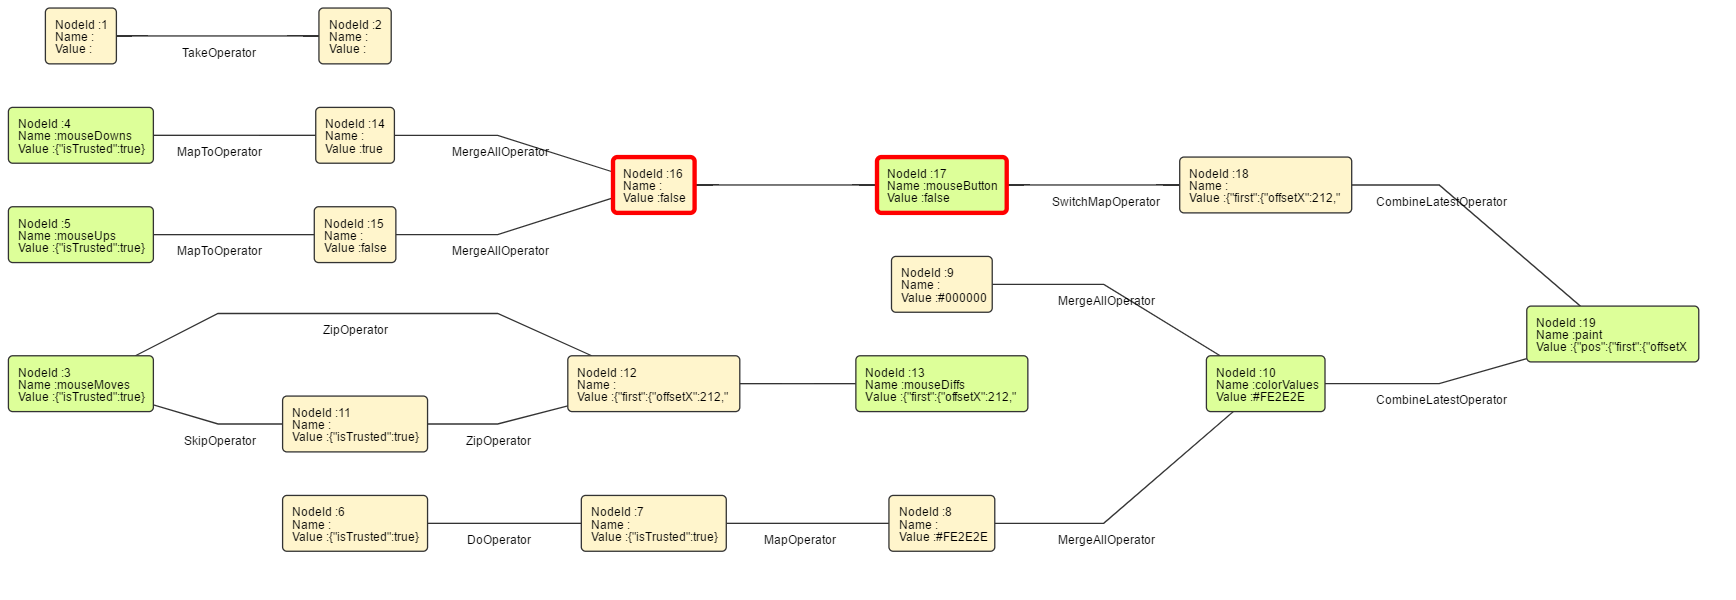
\includegraphics[width=\textwidth,height=\textheight,keepaspectratio]{gfx/evaluation/dgraph_canvaspaint.png}
	\caption{Bacon.js - Dependency Graph of Canvas Painting Board}
	\label{fig:dgraph_canvaspaint}
\end{figure}

\subsection{RxJS - Who to Follow}

The Listing~\ref{lst:evaluation-who_to_follow} shows the relevant part of a \textbf{Who to Follow} application that is based on RxJS. This application imitates the core features of Twitter UI element that suggests other accounts you could follow. Figure~\ref{fig:who_to_follow_dgraph} depicts the GUI of this application. This application loads accounts data from the API on start up and displays three suggestions. When the user clicks on \textbf{Refresh}, it loads three other account suggestions into the three rows. Clicking on the \textbf{x} button on an account row will remove only that current account and display another suggestion. 


\begin{figure}[!h]
	\centering
	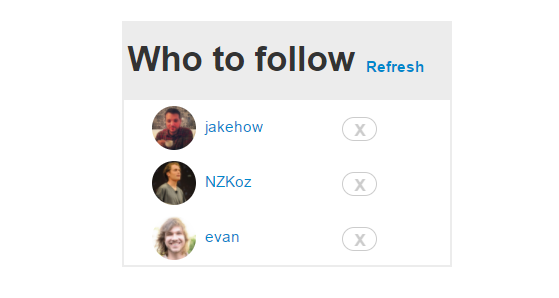
\includegraphics[width=\textwidth,height=\textheight,keepaspectratio]{gfx/evaluation/who_to_follow_ui.png}
	\caption{RxJS - Who to Follow}
	\label{fig:who_to_follow_ui}
\end{figure}

There are five different event streams defined, and five different operators are being used. If we take a closer look into its source code, it seems very short and abstract. It is very hard to understand this kind of abstract code by just looking into the code. We used the CRI extension to get a better understanding of this abstract source code. Figure~\ref{fig:who_to_follow_dgraph} shows the dependency graph generated by the CRI.  The dependency graph and the propagation of changes while interacting with the application gives a broad understanding of the source code of this application. 

\begin{lstlisting}[language=JavaScript, caption=RxJS - Who to Follow, label={lst:evaluation-who_to_follow}]
// UI Elements Selectors
var refreshButton = document.querySelector('.refresh');
var closeButton1 = document.querySelector('.close1');
var closeButton2 = document.querySelector('.close2');
var closeButton3 = document.querySelector('.close3');
// Click Streams
var refreshClickStream = Rx.Observable.fromEvent(refreshButton, 'click');
var close1ClickStream = Rx.Observable.fromEvent(closeButton1, 'click');
var close2ClickStream = Rx.Observable.fromEvent(closeButton2, 'click');
var close3ClickStream = Rx.Observable.fromEvent(closeButton3, 'click');
// Request Stream
var requestStream = refreshClickStream.startWith('startup click')
.map(function() {
	var randomOffset = Math.floor(Math.random()*500);
	// Just so we don't max out the anonymous github api req
	// limit, I've cached a page. We'll pretend for now.
	// To really hit the API, use
	// 'https://api.github.com/users?since=' + randomOffset;
	return 'users.json'
});
// Response Stream
var responseStream = requestStream
.flatMap(function (requestUrl) {
	return Rx.Observable.fromPromise($.getJSON(requestUrl));
});
// Create Suggestion Stream
function createSuggestionStream(closeClickStream) {
	return closeClickStream.startWith('startup click')
	.combineLatest(responseStream,             
	function(click, listUsers) {
		return listUsers[Math.floor(Math.random()*listUsers.length)];
	}
	)
	.merge(
	refreshClickStream.map(function(){ 
		return null;
	})
	)
	.startWith(null);
}
// Creating Streams
var suggestion1Stream = createSuggestionStream(close1ClickStream);
var suggestion2Stream = createSuggestionStream(close2ClickStream);
var suggestion3Stream = createSuggestionStream(close3ClickStream);

// Rendering
function renderSuggestion(suggestedUser, selector) {
	var suggestionEl = document.querySelector(selector);
	if (suggestedUser === null) {
		suggestionEl.style.visibility = 'hidden';
	} else {
		suggestionEl.style.visibility = 'visible';
		var usernameEl = suggestionEl.querySelector('.username');
		usernameEl.href = suggestedUser.html_url;
		usernameEl.textContent = suggestedUser.login;
		var imgEl = suggestionEl.querySelector('img');
		imgEl.src = "";
		imgEl.src = suggestedUser.avatar_url;
	}
}
// Subscription to Steams
suggestion1Stream.subscribe(function (suggestedUser) {
	renderSuggestion(suggestedUser, '.suggestion1');
});
suggestion2Stream.subscribe(function (suggestedUser) {
	renderSuggestion(suggestedUser, '.suggestion2');
});
suggestion3Stream.subscribe(function (suggestedUser) {
	renderSuggestion(suggestedUser, '.suggestion3');
});	
\end{lstlisting}

\begin{sidewaysfigure}[ht]
	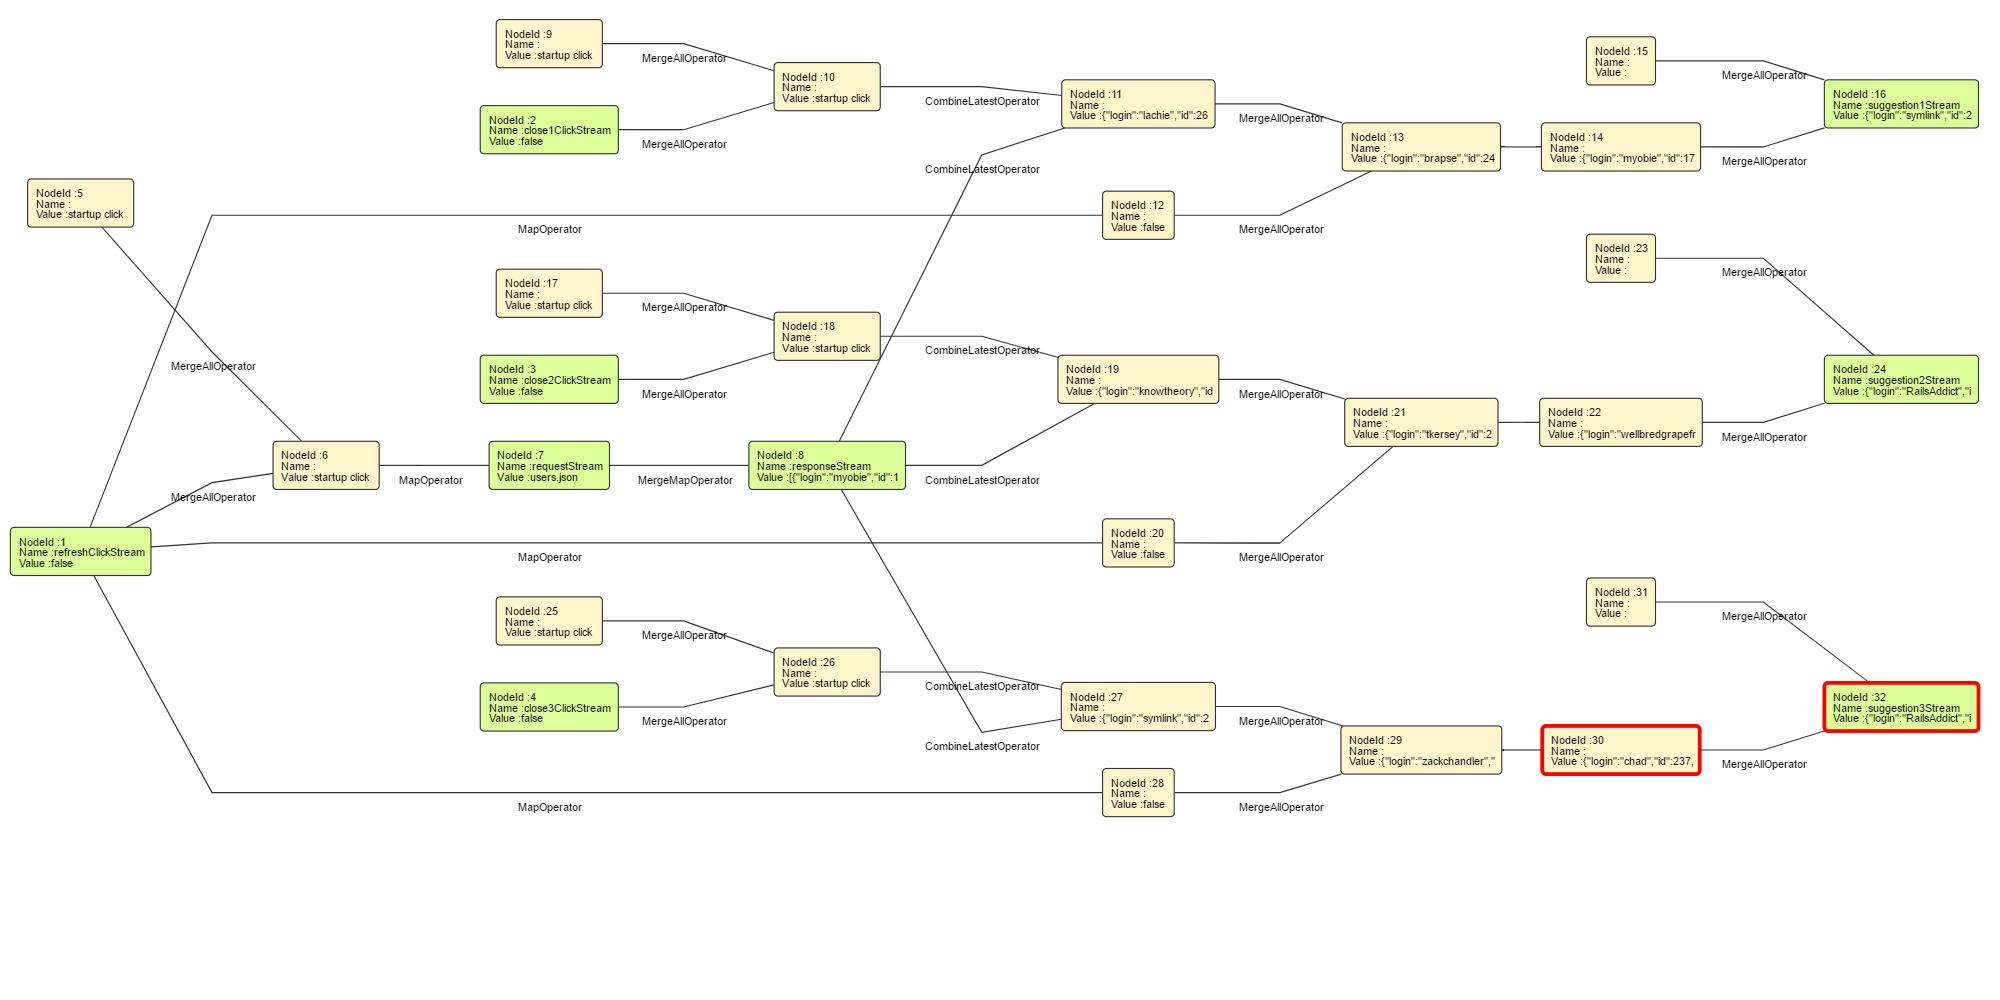
\includegraphics[width=\textwidth]{gfx/evaluation/who_to_follow_dgraph.png}
	\caption{RxJS - Dependency Graph of Who to Follow}
	\label{fig:who_to_follow_dgraph}
\end{sidewaysfigure}





\subsection{Baon.js - Drawing Bar Chart}

\begin{figure}[!h]
	\centering
	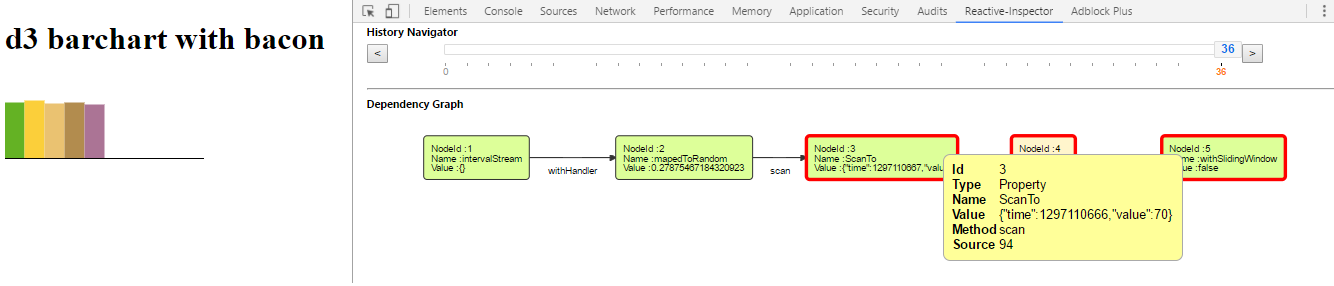
\includegraphics[width=\textwidth,height=\textheight,keepaspectratio]{gfx/evaluation/bar_chart_ui_n_dgraph.png}
	\caption{Bacon.js - UI and Dependency Graph of Drawing Bar Chart}
	\label{fig:bar_chart_ui_n_dgraph}
\end{figure}

\begin{lstlisting}[language=JavaScript, caption=Bacon.js -Drawing Bar Chart, label={lst:evaluation-drawing_bar_chart}]
var initial = {
	time: 1297110663,
	value: 70
}

function walk(prev, rand) {
	return {
		time: prev.time + 1,
		value: ~~Math.max(10, Math.min(90, prev.value + 10 * (rand - .5)))
	};
}

var intervalStream = Bacon.interval(15000);
var mapedToRandom = intervalStream.map(Math.random);
var ScanTo = mapedToRandom.scan(initial, walk);
var withSlidingWindow = ScanTo.slidingWindow(10)
withSlidingWindow.onValue(redraw);
\end{lstlisting}

\textbf{Drawing bar chart} is an application based on Bacon.js, which draws bar chart to the target web page. After every 15000 milliseconds, it adds a bar to the chart with random height. 
The Listing~\ref{lst:evaluation-who_to_follow} shows the relevant code of the target application. Figure~\ref{fig:bar_chart_ui_n_dgraph} is a screenshot of a debugging session with this application, where the left side depicts the GUI of the application, and the right side shows the dependency graph. With the passage of time, we can observe the values emitted by observables by hovering over the nodes of the dependency graph.




\subsection{Bacon.js - Live Wikipedia Updates Over Websockets}

\begin{figure}[!h]
	\centering
	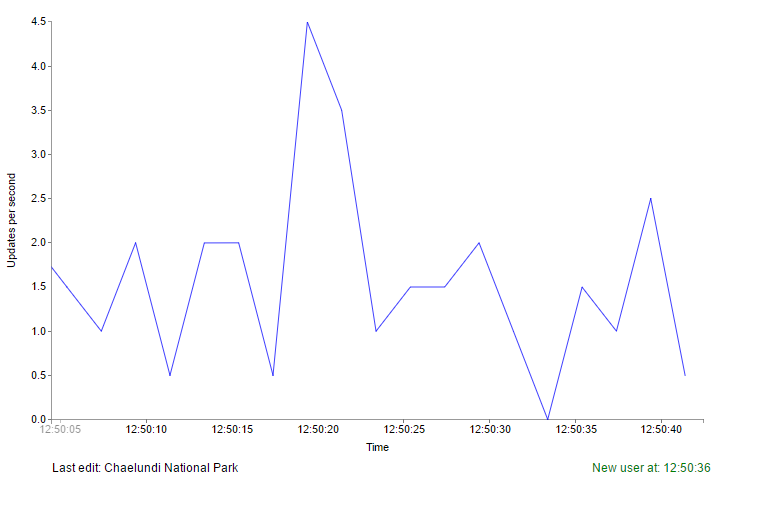
\includegraphics[width=\textwidth,height=\textheight,keepaspectratio]{gfx/evaluation/w_pedia_updates_over_websocket_ui.png}
	\caption{Bacon.js - Live Wikipedia Updates Over Websockets}
	\label{fig:w_pedia_updates_over_websocket_ui}
\end{figure}

\begin{lstlisting}[language=JavaScript, caption=Bacon.js - Live Wikipedia Updates Over Websockets, label={lst:evaluation-w_pedia_updates_over_websocket}]

// Create our websocket to get wiki updates
var ws = new WebSocket("ws://wiki-update-sockets.herokuapp.com/");
var updateStream = Bacon.fromEventTarget(ws, "message").map(function(event) {
	var dataString = event.data;
	return JSON.parse(dataString);
});

// Filter the update stream for newuser events
var newUserStream = updateStream.filter(function(update) {
	return update.type === "newuser";
});
newUserStream.onValue(function(results) {
	var format = d3.time.format("%X");
	updateNewUser(["New user at: " + format(new Date())]);
});

// Filter the update stream for unspecified events, which we're taking to mean 
// edits in this case
var editStream = updateStream.filter(function(update) {
	return update.type === "unspecified";
});
editStream.onValue(function(results) {
	updateEditText(["Last edit: " + results.content]);
});

// Calculate the rate of updates over time
var updateCount = updateStream.scan(0, function(value) {
	return ++value;
});

var sampledUpdates = updateCount.sample(samplingTime);
var rateUpdates = sampledUpdates
					.map(function (value) {
						// timestamp all samples
						return {date: new Date(), value: value};
					})
					.slidingWindow(2)
					.skip(2) // we'll ignore the first two results, they don't contain enough samples to determine a rate
					.map(function(updates) {
						// Determine rate of the last two samples
						var previous = updates[0];
						var current = updates[1];
						return {
							x: current.date,
							y: (current.value - previous.value) / (current.date - previous.date) * 1000 // Delta is in ms, but we need s.
						}
						//
					});

var graphtData = rateUpdates
.slidingWindow(maxNumberOfDataPoints)
.onValue(function (updates) {
	update(updates)
});
\end{lstlisting}

Listing~\ref{lst:evaluation-w_pedia_updates_over_websocket} shows an excerpt from a Bacon.js application that creates a websocket connection to third party server. This websocket connection receives messages that contain different types of update notifications from Wikipedia. The stream of recieved messages is converted into EventStresm named as \textbf{updateStream}. Target application filter \textbf{updateStream} further into three streams, which are \textbf{newUserStream}, \textbf{editStream} and \textbf{updateCount}. These filtered streams are used to create a graph that updates on the fly and updates other information to the target web page. Figure~\ref{fig:w_pedia_updates_over_websocket_ui} and ~\ref{fig:dgraph_wpedia_updates} shows the GUI and dependency graph of the target application.


\begin{figure}[!h]
	\centering
	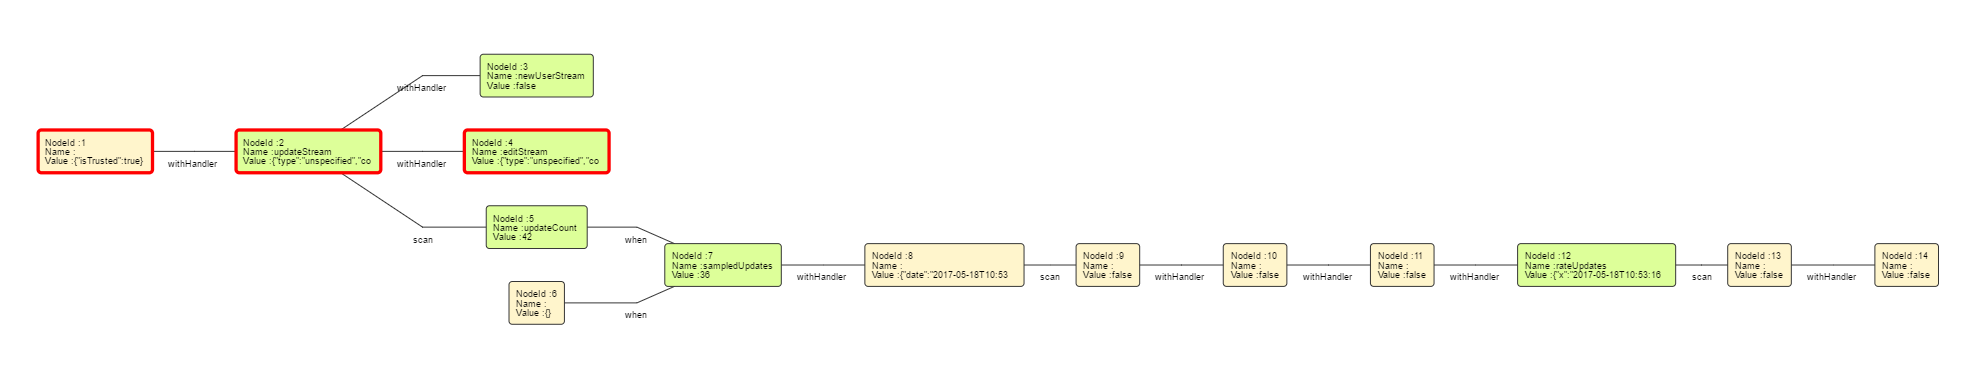
\includegraphics[width=\textwidth,height=\textheight,keepaspectratio]{gfx/evaluation/dgraph_wpedia_updates.png}
	\caption{Bacon.js - Dependency Graph of Live Wikipedia Updates Over Websockets}
	\label{fig:dgraph_wpedia_updates}
\end{figure}

\section{Summary of the Evaluation}
While these case studies do not prove the CRI extension\textquotesingle s performance, they demonstrate its usefulness when debugging real web applications containing reactive code. In these case studies, the user was able to get a better grasp of the internal workings of the target application while quickly viewing the dependency graph and being able to navigate through the history of the dependency graph. 
These case studies indirectly present some of the deficiencies of the CRI extension as well. Firstly, if the target application has some event streams that emits values after a very short time interval, this can be very resource and memory consuming. Secondly, if the target application code contains arrow functions syntax, then it might not work because Jalangi does not support it.
The CRI extension offers powerful tools, demonstrated in these case studies, that could make the CRI more efficient than native DevTools. Our extension works fine with most of the applications we took from the internet, and we are confident to say that the technical approach we have used would work more accurately with a little bit of fine tuning.